% Performance evaluation
% Benchmark de Dani
% Robar algo de la tesis de Dani para comentar sobre el benchmark?
% Comparación con la versión previa
% Gráficos dcs vs dcs 2, dcs2 vs las otras herramientas

Para realizar las pruebas de performance decidimos usar el mismo conjunto de problemas que el utilizado para examinar el algoritmo original de \DCS en \cite{tesisDani}. En esta sección presentamos los resultados de la comparación versus dicha versión y, además, contra diversos programas del estado del arte. Todos los casos de estudios fueron escritos con la posibilidad de ser escalados en el número de componentes y estados.
\begin{description}
    \item [Transfer Line] Automatización de una fábrica, un dominio de mucho interés en el área de supervisory control. TL consiste de n máquinas conectadas por $n$ buffers cada uno con capacidad de $k$ unidades, termina en una máquina adicional llamada Test Unit.
    
    \item [Dinning Philosophers] Problema clásico de concurrencia. En DP hay $n$ filósofos sentados en una mesa redonda, cada uno comparte un tenedor con sus vecinos aledaños. El objetivo del sistema es controlar el acceso a los tenedores de manera que los filósofos puedan alternar entre comer y pensar; evitando \textit{deadlock} y \textit{starvation}. Adicionalmente, cada filósofo, luego de tomar un tenedor, debe cumplir con $k$ pasos de etiqueta antes de comer.

    \item [Cat and Mouse] Juego de dos jugadores donde cada uno toma turnos para moverse a una casilla adyacente dentro de un mapa de la forma de un corredor dividido en $2k + 1$ áreas. En CM $n$ gatos y la misma cantidad de ratones son colocados en extremos opuestos del corredor. El objetivo es mover a los ratones de manera que no terminen en el mismo lugar que un gato. Los movimientos de los gatos no son controlables. En el centro del corredor hay un agujero que lleva a los ratones a un área segura.
    
    \item [Bidding Workflow] Modela el proceso de evaluación de proyectos de una empresa. El proyecto debe ser aprobado por $n$ equipos. El objetivo es sintetizar un flujo de trabajo que intente llegar a un consenso, es decir, aprobar/rechazar el proyecto cuando todos los equipos lo aceptan/rechazan. La propuesta puede ser reasignada para re-evaluación por un equipo hasta $k$ veces, no se puede reasignar si el equipo ya lo había aceptado. Cuando un equipo lo rechaza $k$ veces el proyecto puede ser rechazado sin consenso. Es un caso de estudio típico del dominio de Business Process Management.
    
    \item [Air-Traffic Management] Representa la torre de control de un aeropuerto, que recibe $n$ peticiones de aterrizaje simultáneas. La torre necesita avisar si tiene permiso para aterrizar o, en caso contrario, en cuál de los $k$ espacios aéreos debe realizar maniobras de espera. El objetivo es que todos los aviones puedan aterrizar de manera segura. El problema solo tiene solución si la cantidad de aviones es menor a la de espacios aéreos ($n<k$).
    
    \item [Travel Agency] Modela una página on-line de ventas de paquetes de viajes. El sistema depende de $n$ servicios de terceros para realizar las reservas (ej. alquiler de auto, compra de pasajes, etc). Los protocolos para utilizar los servicios pueden variar de manera no controlable; una variante es la selección de hasta $k$ atributos (ej. destino del vuelo, clase y fechas). El objetivo del sistema es orquestar los servicios de manera de obtener un paquete de vacaciones completo de ser posible, evitando pagar por paquetes incompletos.
\end{description}

\section{Comparación con versión previa de \DCS}
Como ya dijimos, el foco del trabajo no estuvo solo en corregir los errores encontrados en el algoritmo sino también en brindar una mayor seguridad sobre la corrección y completitud de la exploración on the fly. Esto debía hacerse sin perder la buena performance que aportaba la técnica, permitiendo aplicarla a casos de mayor tamaño. Aclaramos que el benchmark se corrió en un equipo de las mismas características para ambas versiones de \DCS.

La comparación se realizó para las dos heurísticas desarrolladas en \cite{tesisDani}, Monotonic Abstraction y Ready Abstraction. Agregamos además una de las heurísticas naif, BFS, que desarrollamos para depurar el código; esto es en función de mostrar la posible ganancia obtenida a través de una buena heurística.

\begin{figure}[th]
    \centering
    \hspace*{-20mm}
    \begin{subfigure}{0.7\textwidth}
        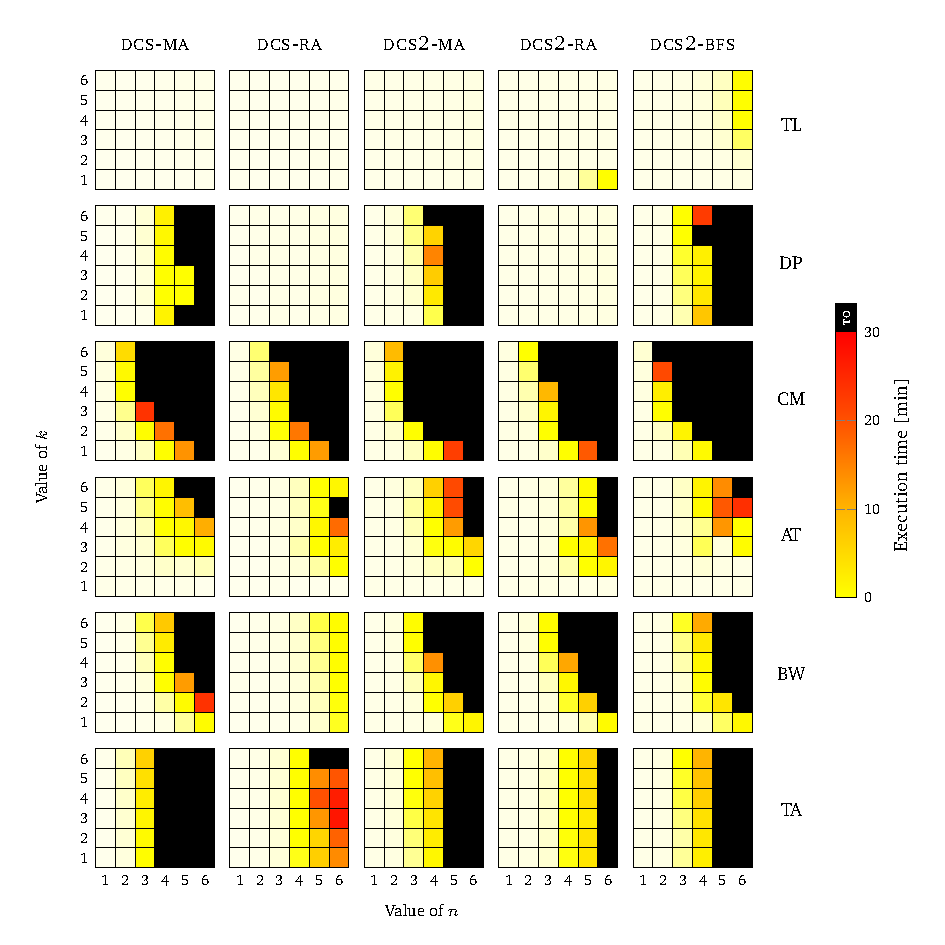
\includegraphics[width=\linewidth]{figures/benchmark/dcs_vs.pdf}\label{fig:dcs:results:detailed}
        \caption{\DCS detailed benchmark results.}
    \end{subfigure}%
    \begin{subfigure}{0.5\textwidth}
        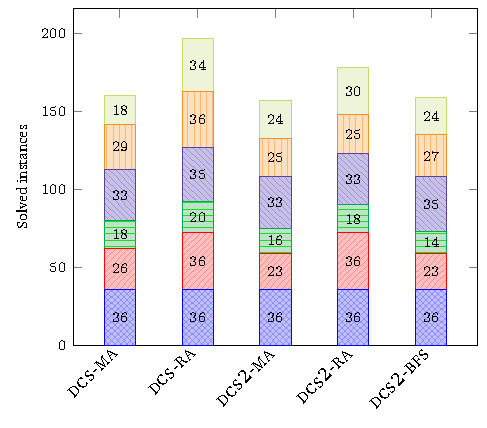
\includegraphics[width=0.9\linewidth]{figures/benchmark/dcs_instances.pdf}\label{fig:dcs:results:instances}
        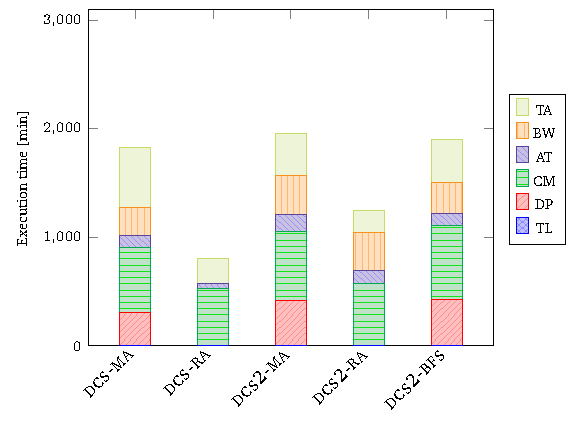
\includegraphics[width=\linewidth]{figures/benchmark/dcs_time.pdf}\label{fig:dcs:results:time}
        \caption{Total solved instances (top) and execution time (bottom) with \DCS.}
    \end{subfigure}
\caption{Benchmark results.}
\label{fig:dcs:results}
\end{figure}

En la figura~\ref{fig:dcs:results} se pueden observar los resultados con respecto a DCS anterior. Antes que nada podemos concluir que hay una ganancia al utilizar mejores heurísticas, ya que BFS pierde contra RA tanto en cantidad de instancias como tiempo. Sorprendentemente a pesar de ser muy naif termina compitiendo contra MA. Esto se puede deber a la estructura de los problemas y la forma de cerrar estados, BFS estaría intentando llegar a una conclusión dentro de una localidad antes de mirar más lejos.

Nuestra versión (dcs2) mantiene la performance en la mayoría de los casos de estudio. En TA hay algunas instancias nuevas que dan timeout, pero el resto concluyen rápidamente. El único caso donde pierde notoriamente es BW, pero mirando otras herramientas vemos que en general tienen problemas con las combinaciones más grandes (salvo \MYND). Nuestra suposición es que se están cerrando estados como $\Goals$ de manera anticipada y posiblemente erronea, quizás casos como el de \ref{test:goals:falsopositivo}. Esto puede hacer que se llegue a una conclusión apurada que, si bien es correcta porque el problema es controlable, devuelva un controlador incorrecto.

\section{Comparación con otros programas}

Si bien nuestra exploración parece perder un poco de escalabilidad en ciertos casos, en la figura \ref{fig:tools:results} podemos ver que seguimos en una posición competitiva con respecto a otras herramientas del estado del arte. Para que sea más simple la comparación decidimos mostrar solo RA, ya que es la heurística de mejor desempeño, y ambas versiones de \DCS. 

Aunque la nueva versión esté un poco más lejos de \MYND, en calidad de cantidad de intancias y tiempo supera ampliamente el resto de las opciones, referirse a fig \ref{fig:tools:results:instances} y \ref{fig:tools:results:time}.
\begin{figure}[th]
    \centering
    \hspace*{-20mm}
    \begin{subfigure}{0.7\textwidth}
        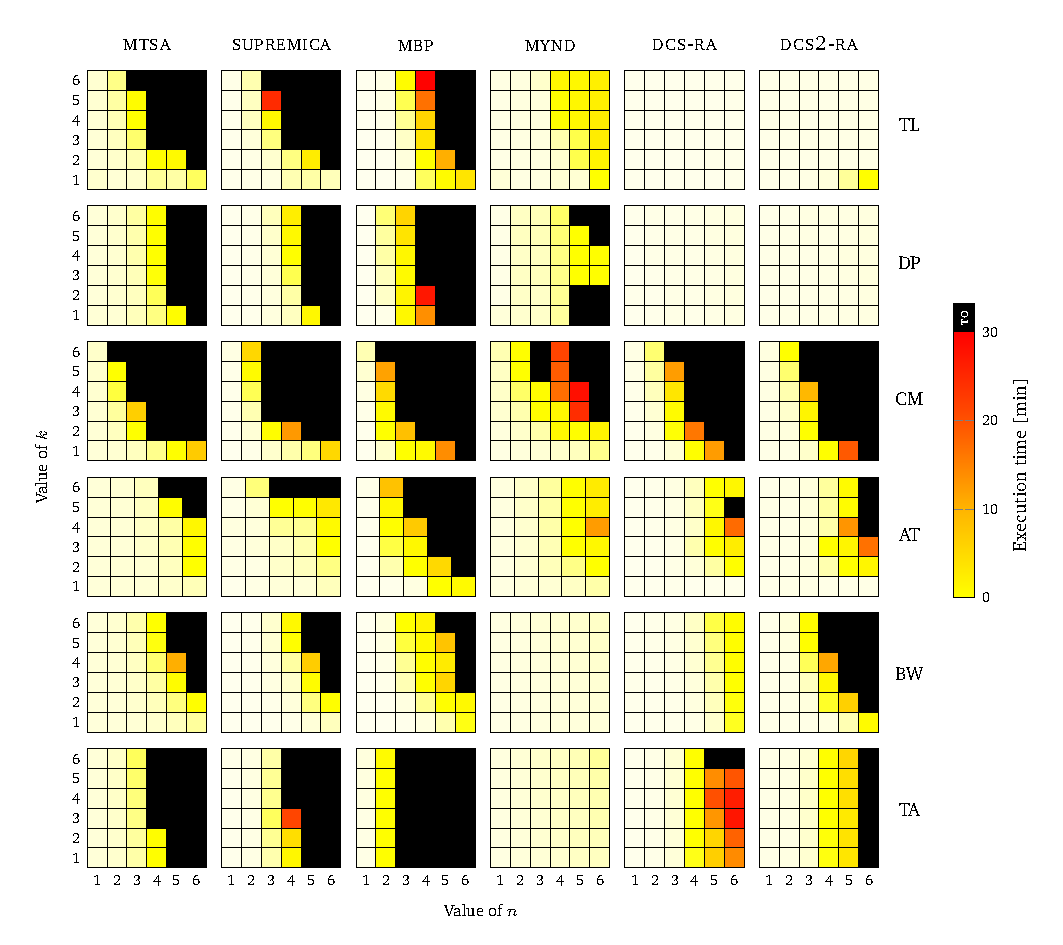
\includegraphics[width=\linewidth]{figures/benchmark/tools_vs.pdf}\label{fig:tools:results:detailed}
        \caption{\DCS detailed benchmark results.}
    \end{subfigure}%
    \begin{subfigure}{0.5\textwidth}
        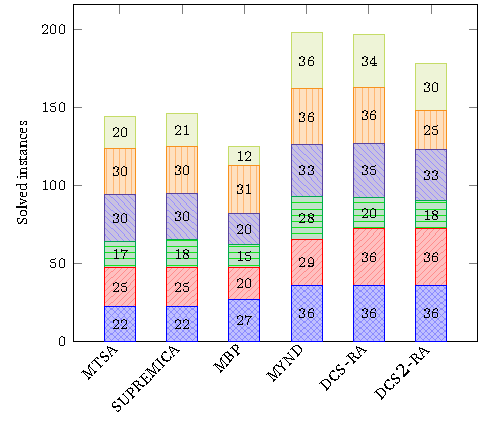
\includegraphics[width=0.9\linewidth]{figures/benchmark/tools_instances.pdf}\label{fig:tools:results:instances}
        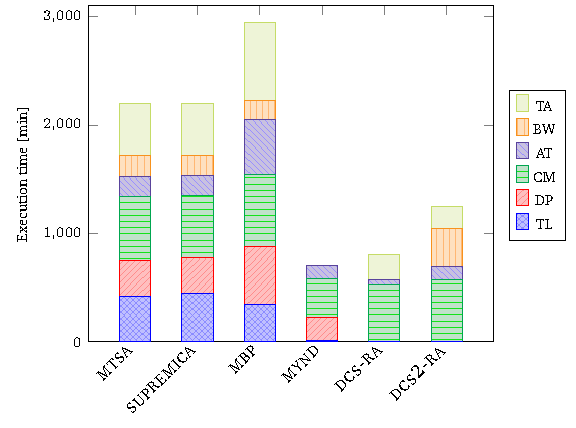
\includegraphics[width=\linewidth]{figures/benchmark/tools_time.pdf}\label{fig:tools:results:time}
        \caption{Total solved instances (top) and execution time (bottom) with \DCS.}
    \end{subfigure}
\caption{Benchmark results.}
\label{fig:tools:results}
\end{figure}
